%%%%
\section{Amostragem}

% http://maps.google.com/maps/ms?ie=UTF8&hl=en&msa=0&msid=116003586198857296821.00046d7e7367b947abe12&z=12

Londrina is a city with 548,000 inhabitants located in the
state of Paraná, southern Brazil (lat. 23°19%′S, long. 51°08′W,
alt. 630 m). It was founded in 1934 and despite being a young
city, Londrina faces environmental problems comparable toda
older and larger cities in the country. The motorized fleet
grew 85% in the last decade, and is dominated by passenger
vehicles (78.3%) that circulate with an average of 1.47
persons per vehicle. Motorcycles increased 67.6% in the
period 2005–2014 as an affordable alternative to the
inefficient public transportation system. The motorization
rate reached 661 vehicles per 1000 inhabitants in June
2015, which is much higher than the national rate (436
vehicles per 1000 inhabitants). Londrina has a humid
subtropical climate (Cfa in the Köppen–Geiger classification)
with an annual mean temperature of 21.0°C and annual
mean precipitation of 1,630 mm. Rainfall occurs throughout
the year, but mostly in the summer (December to February)
whereas winters are drier. In winter, the average air
temperature (T air ) and relative humidity (RH) range from
11.6 to 25.8°C, and 62 to 75%, respectively, and from 19.0
to 29.7 C, and 72 to 77% in summer. Insolation is greatest
during winter time (mean value of 225 h) when cloud
coverage is lowest (Targino et al., 2014).

he measurements were conducted in the dry and
wet months to capture different patterns of BC concentrations
governed not only by sources typically found in urban
environments (e.g., traffic emissions), but also by sporadic

(e.g., open backyard burning) and seasonal (LRT) emissions.
A description of the measurement sites follows and their
geographical location is displayed in Fig.1

The UTF campus is located ca. 8 km from Londrina’s
city center, on the eastern edge of the city, with the closest
neighborhood consisting of sparsely built, detached houses
about 400 m away, across wheat and soybean fields. The
major motor vehicle pollution source comes from a paved
road which gives access to the campus and to a residential
cluster development, with a traffic volume of 2,700
vehicles day –1 on weekdays (8.4\% are diesel heavy-duty
vehicles). The measurement site is located 165 m from this
road in straight line. Visual inspection indicates that open
fires occur frequently near the campus during the dry season
when residents burn branches, leaves, domestic debris and
also plastic from copper wiring.

This is a 2.8-km arterial road aligned in the north-south
direction and collects traffic from many small streets, crossing
areas of commercial buildings and high-rise multifamily units.
The road has two lanes in each direction and lies on terrain
with varying heights (maximum elevation difference of 100
m). The daily traffic volume amounts to ~25,000 vehicles day –1
on weekdays (2.4% are diesel heavy-duty vehicles) and up
to 3,700 vehicles h –1 in the evening rush hours.

Sergipe is a heavily-trafficked one-way street aligned in
the east-west direction, located in the city center, with intense
commercial activity from Monday to Saturday. Measurements
took place within a flat transect that presents a canyon
structure (width of 14.5 m and length of 113 m), with
buildings continuously flanking both sides of the street with
heights between 3.9 and 9.7 m. The traffic is organized in
two lanes with a speed limit of 40 km h –1 , and controlled
by traffic lights situated at both ends of the transect. Thus,
start-stop driving is the general driving pattern and congestion
is frequently observed during rush hours. Manual counting
conducted at specific times revealed a traffic rate of 1,050
vehicles h –1 in the afternoon, with the following share:
passenger cars and light-duty vehicles (66.6%), motorcycles
(24.0%), buses (7.8%) and trucks (1.6%).

A campanha de amostragem ocorreu em Acra (capital de Gana) 
entre 11 de Novembro de 2006 e 15 de Agosto de 2008. 
Foram coletadas 879 amostras de 48 horas no topo de duas residências 
no bairro de \textbf{Nima}.

Os dois pontos de amostragem distam entre si 280 metros, sendo um na rua
\textbf{Sam Rd} com característica residencial
(+5$\degree$ 35$'$ 2$''$,-0$\degree$ 11$'$ 58$''$)
e o outro na avenida \textbf{Al-Waleed bin Talal Highway} 
(+5$\degree$ 34$'$ 54$''$, -0$\degree$ 11$'$ 56.3$''$) com comércios e
alta movimentação veículos, pois conecta diversos bairros ao centro
\ref{fig:nima}. 

\begin{figure}[H]
\begin{center}
  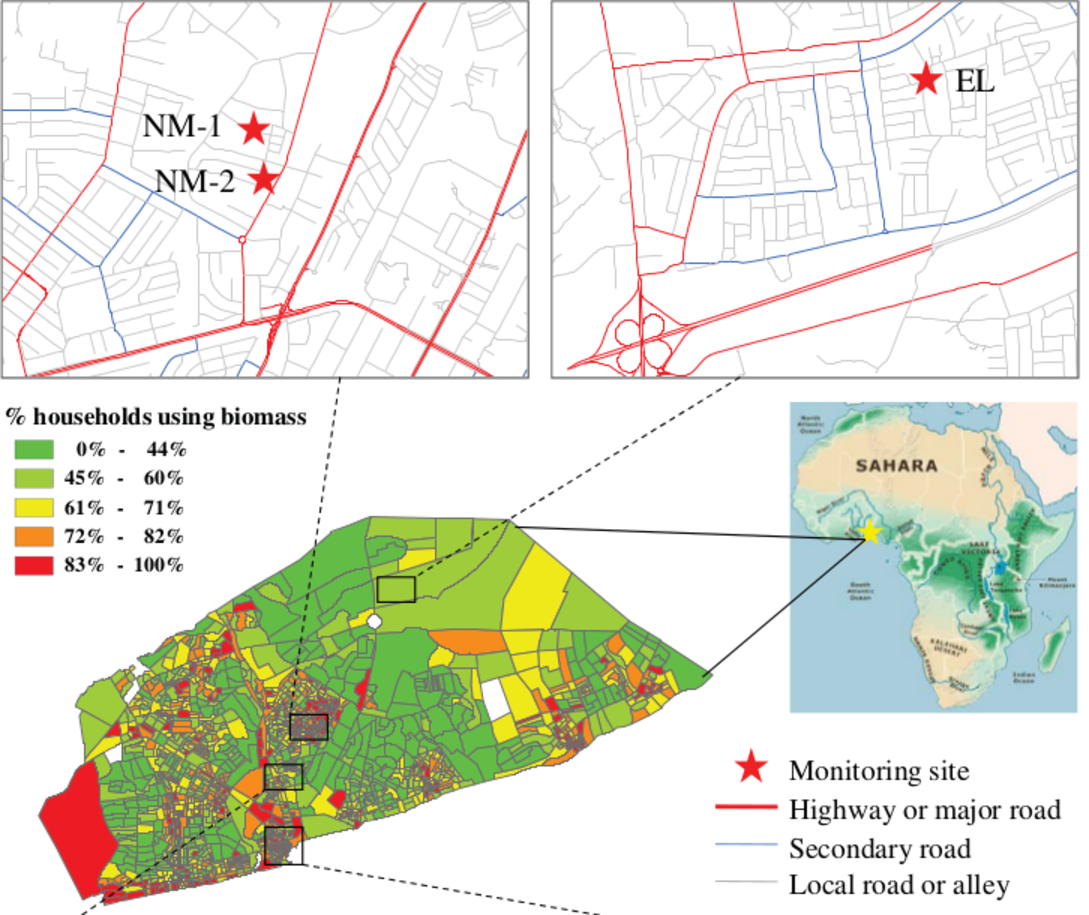
\includegraphics[width=0.6\textwidth]{../inputs/images/zheng/nima_mapa.pdf}
  \caption{Mapa de Nima. NM-1 ponto de amostragem na área residencial e 
           NM-2 ponto de amostragem na avenida. Porcentagem do uso da queima
           de biomassa para preparação de alimentos em residências usando dados
           do censo de 2000 \citep{ghanacensus2003} \label{fig:nima_mapa}}
\end{center}
\end{figure}

A coleta foi diária, mas houve dias sem medidas devido a falta de eletricidade,
problemas no amostrador, filtros danificados, ausência do operador, entre outros. 

Concentrações dos poluentes variam ao longo do dia na atmosfera
e quanto menor o tempo de amostragem, se obtém melhor resolução 
para identificação das fontes. Porém, amostras com concentrações menores, 
são mais difíceis de se medir devido ao limite de detecção dos equipamentos
\citep{calzolai2015}. 12 ou menos horas de amostragem permitiria captar 
a variabilidade das fontes de Acra (por ser uma região muito poluída).
Mas, o tempo de amostragem foi de 48 horas, e foi definido antes da 
entrada \textbf{USP} no projeto.

As amostras  foram coletadas em filtro de Teflon do tipo 
\textbf{PTFE} de 37 $mm$ de diâmetro, com orifícios de 0,2 $\mu m$ de diâmetro. 

%TODO: qual método foi utilizado para medir a área?
A área de deposição nos filtros foi de $7,32 (\pm 0,366) cm^2$ .

Impactadores são responsáveis pela coleta e classificação 
do material particulado, utilizando-se para tal a inercia das
partículas.
Para $MP_{10}$ utilizou-se impactador Harvard com $D_{50}$ de $10 \mu m$ 
com fluxo de $10,0 L/min$ \citep{marple1987}. 

Nas medidas de $MP_{2,5}$, também utilizou-se impactador Harvard, 
mas com $D_{50}$ de $2,5 \mu m$ acoplado com um \textbf{inlet} 
responsável fazer a filtragem de $MP_{2,5}$.

Os volumes amostrados foram medidos por um integrador de volume
com 5\% de incerteza.

Filtros brancos de campo e laboratórios foram separados para avaliar 
possíveis contaminações no tranporte e manipulação das amostras. 

O laboratório da \textbf{Harvard School of Public Health} foi
utilizado para pesagem das amostras.

Os filtros foram pesados antes e depois da amostragem, usando uma balança 
microanalítica \textbf{(Mettler Toledo MT5)} com precisão de $1 \mu g$, 
seguindo procedimentos padrões de controle de umidade ($39 \pm 2 \%$), 
temperatura ($20,5 \pm 0,2 ^{\circ} C$) e eliminação de cargas eletrostáticas 
(fonte de polônio). 
Cada medida de pesagem foi realizada duas vezes e o valor final foi a média das 
duas medidas. 
